\def \statemodule {MotionEstimation}
\def \handleevent {Алгоритм обработки событий}



\section{Проектирование программного средства}
\subsection{Датчики}
В качестве поддерживаемых датчиков было выбрано три ключевых:
\begin{itemize}
	\item 2D Lidar;
	\item IMU;
	\item GPS.
\end{itemize}

Эти датчики обеспечивают систему данными о пространстве, в котором находится
робот, его ориентации и глобальном местоположении.
2D Lidar позволяет получать информацию о препятствиях вокруг устройства, IMU
предоставляет данные о наклоне и угловых ускорениях, а GPS — о глобальной
позиции робота. Все эти данные интегрируются в систему навигации, создавая
основу для безопасного и эффективного перемещения устройства в различных
условиях.

2D Lidar (Light Detection and Ranging) работает на основе принципа измерения
расстояния до объектов с использованием лазерных импульсов. Ли дар излучает
лазерные импульсы, которые отражаются от объектов, встречающих их на пути.
Время, которое требуется импульсу для прохождения от лидара до объекта и
обратно, используется для вычисления расстояния до объекта. Этот процесс
повторяется многократно по всей области сканирования, создавая карту расстояний
на основе измерений.

\begin{figure}[h]
\centering
	\fbox{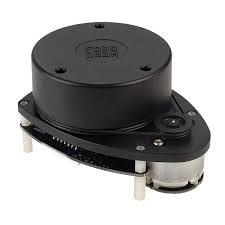
\includegraphics[width=9cm]{2d_lidar}}
\caption{2D Lidar}
\end{figure}

2D лидары обычно работают в плоскости, что означает, что они измеряют расстояния
только в одном направлении (по горизонтали или вертикали). Сканер вращается или
перемещается по оси, чтобы покрыть широкую область, создавая двумерное
изображение окружающего пространства. С помощью таких данных система может
строить карту и распознавать объекты, определяя их положение и расстояние до
них, что крайне важно для навигации роботов и беспилотных автомобилей.

IMU (Inertial Measurement Unit) — это датчик, который измеряет и сообщает
информацию о движении и ориентации объекта в пространстве. Он состоит из трех
основных компонентов: акселерометров, гироскопов и иногда магнитометров.
Акселерометры измеряют ускорения по трем осям (X, Y, Z), что позволяет
определить изменение скорости и положение объекта относительно земной
гравитации. Гироскопы отслеживают угловые скорости вращения вокруг тех же осей,
что помогает измерять ориентацию объекта и его вращения. Магнитометры, если они
присутствуют, измеряют магнитное поле Земли, что позволяет дополнительно
корректировать ориентацию.

Принцип работы IMU заключается в интеграции данных с этих сенсоров, чтобы
получить полное представление о движении и положении объекта. Например,
акселерометры могут обнаружить, если устройство наклоняется или ускоряется, а
гироскопы отслеживают угловые изменения, такие как вращение вокруг своей оси.
Это позволяет системе вычислить изменения ориентации и траекторию движения, что
полезно в таких приложениях, как робототехника, авиация и навигация в условиях
отсутствия GPS.

GPS — это навигационная система, основанная на использовании спутников для
определения местоположения объектов на Земле. Система состоит из спутников,
находящихся на орбите, наземных станций и приемников, которые используются для
получения данных о местоположении. Спутники передают сигналы с точным временем,
и приемник на Земле, получая эти сигналы от нескольких спутников, может
вычислить свое местоположение.

Принцип работы GPS заключается в измерении времени, которое требуется сигналу,
чтобы добраться от спутника до приемника. Поскольку спутники известны своей
точной орбитой, приемник может определить расстояние до каждого спутника,
используя это время. Получая сигналы от как минимум четырех спутников, приемник
может точно вычислить свою абсолютную позицию в трехмерном пространстве —
определяя широту, долготу и высоту, а также время. Эти данные обеспечивают
высокую точность определения местоположения, что критически важно для навигации
и локализации в реальном времени.


\subsection{Проектирование архитектуры}	

После того, как были сформулированы функциональные требования к разрабатываемой
системе,  а  также  исходя  из  результатов  анализа  существующих
программных решений, можно определить основные моменты организации системы,  в
которой  будет  функционировать  разрабатываемое  программное  решение.

Процесс проектирования архитектуры программного обеспечения включает в себя сбор
требований, их анализ и создание проекта для компонента программного
обеспечения в соответствие с требованиями. Успешная разработка ПО должна
обеспечивать баланс неизбежных компромиссов вследствие противоречащих
требований;  соответствовать  принципам  проектирования  и  рекомендованным
методам,  выработанным  со  временем;  и  дополнять  современное оборудование,
сети и системы управления. 

Архитектуру  программного  обеспечения  можно рассматривать  как  сопоставление
между целью компонента ПО и сведениями о реализации в коде. Правильное понимание
архитектуры  обеспечит  оптимальный баланс требований и результатов. Только
программное обеспечение с хорошо продуманной архитектурой способно выполнять
указанные задачи с параметрами исходных требований, одновременно обеспечивая
максимально высокую производительность. Программное средство построено на основе
модульной архитектуры. 

\FloatBarrier
\begin{figure}[H]
\centering
	\fbox{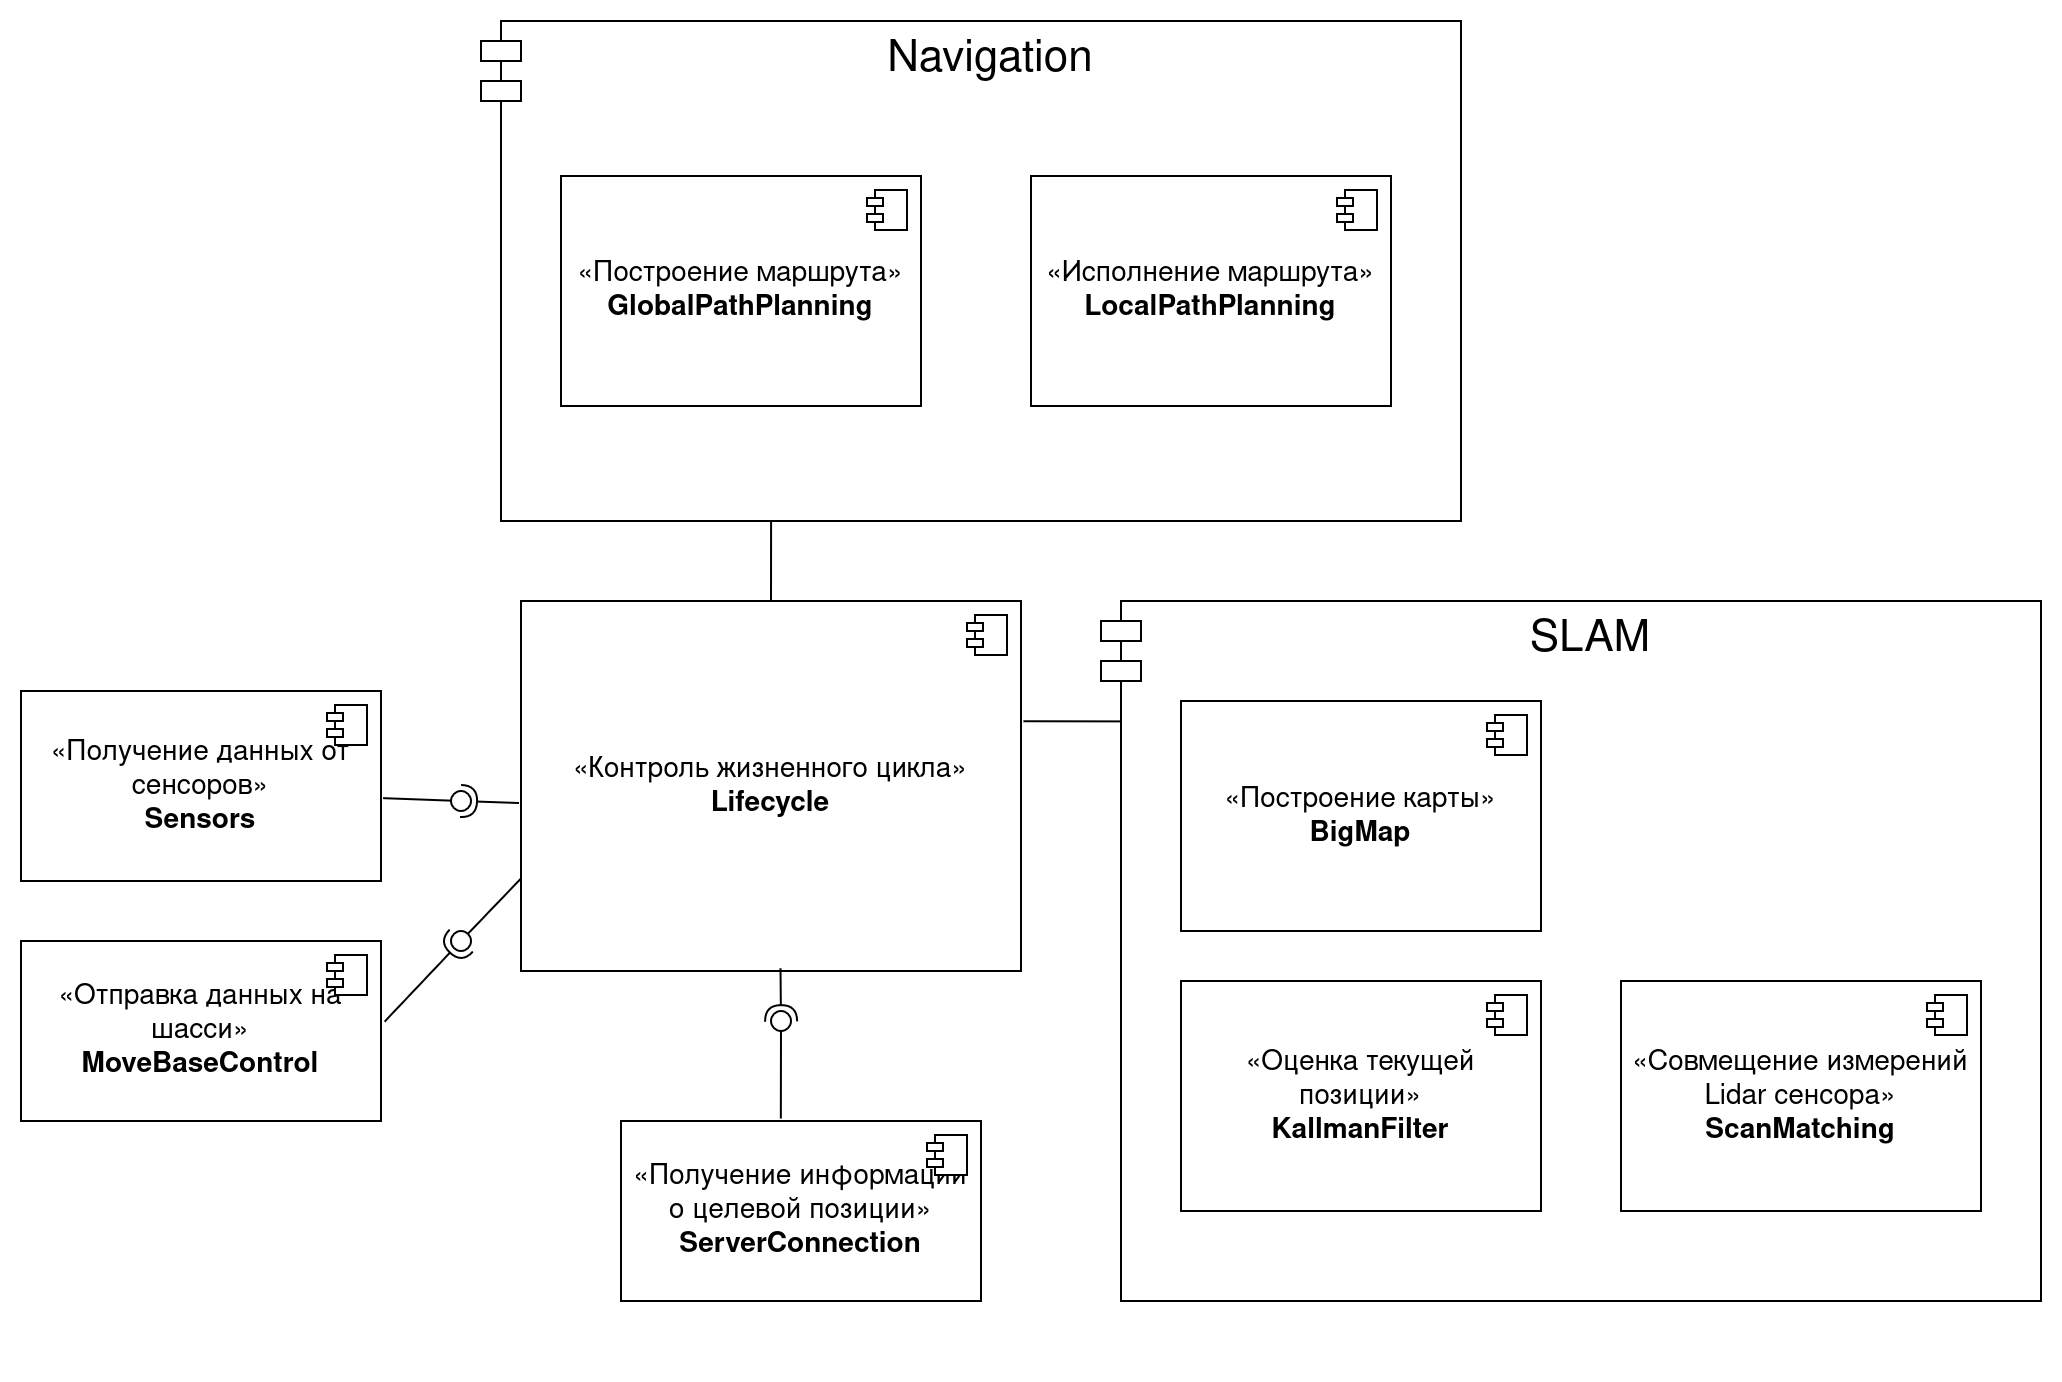
\includegraphics[width=15cm]{MODULES.drawio}}
\caption{Диаграмма компонентов проектируемого ПО}
\label{fig:components}
\end{figure}

На рисунке \ref{fig:components} отображены модули системы:~
\begin{itemize}
	\item модуль жизненного цикла;
	\item модуль построения маршрута;
	\item модуль исполнения маршрута;
	\item модуль получения данных сенсоров;
	\item модуль отправки данных на шасси;
	\item модуль получения информации о целевой позиции;
	\item модуль построения карты;
	\item модуль оценки позиции;
	\item модуль совмещения измерений Lidar сенсора.
\end{itemize}

\subsection{CSM}
Correlative scan matching (CSM) — это метод регистрации сканов лидара, используемый в робототехнике для определения относительного положения робота на карте. Его ключевое преимущество — устойчивость к локальным минимумам и высокая точность, что делает его критически важным для задач одновременной локализации и построения карт (SLAM).

Принцип работы CSM заключается в поиске оптимального преобразования (сдвига и поворота) между двумя наборами точек (сканами), при котором достигается максимальное совпадение между ними. В отличие от итеративных методов, таких как ICP (Iterative Closest Point), которые зависят от начального приближения и могут застревать в локальных оптимумах, CSM осуществляет дискретный перебор возможных трансформаций в заданном диапазоне. Для каждой трансформации вычисляется функция качества совпадения, основанная на вероятностной модели окружающей среды или на карте стоимости.

Алгоритм строит карту стоимости, где каждой точке пространства соответствует значение, отражающее вероятность её принадлежности к объекту или свободному пространству. Затем, перебирая множество вариантов сдвигов и поворотов, CSM вычисляет суммарную оценку совпадения между текущим сканом и картой. Оптимальное преобразование выбирается как то, при котором эта оценка максимальна.

Преимущества CSM включают:
\begin{itemize}
	\item Глобальный поиск решения, минимизирующий риск сходимости к локальным минимумам.
	\item Высокую устойчивость к шуму и ошибкам сенсорных данных.
	\item Возможность работы при значительной начальной неопределённости положения.
\end{itemize}

CSM широко применяется в задачах одновременной локализации и построения карт (SLAM), особенно для коррекции ошибок одометрии и закрытия петель, что позволяет значительно повысить точность и надёжность навигационных систем мобильных роботов.


\subsection{ICP}

Iterative Closest Point (ICP) — это классический алгоритм регистрации облаков точек, широко используемый в компьютерном зрении и робототехнике для точного выравнивания двух наборов данных, полученных с помощью лидаров или других 3D-сканеров.

Основная цель ICP — минимизировать расстояние между двумя облаками точек: фиксированным эталонным (reference) и подвижным (source), который необходимо трансформировать (сдвинуть и повернуть) так, чтобы максимально приблизить к эталону. Алгоритм работает итеративно, последовательно уточняя параметры преобразования.

\subsubsection{Принцип работы ICP}

1 Алгоритм начинается с предварительной оценки преобразования, которое приблизительно совмещает исходное облако с эталонным. Качество начального приближения существенно влияет на результат, поскольку ICP может сойтись к локальному минимуму.
    
2 Для каждой точки подвижного облака находится ближайшая точка в эталонном облаке по евклидову расстоянию. Для ускорения поиска обычно используется структура данных k-d дерево.
    
3 На основе найденных пар точек вычисляется оптимальное преобразование (смещение и поворот), минимизирующее среднеквадратичное расстояние между соответствующими точками. Часто применяется метод наименьших квадратов.
    
4 Подвижное облако точек трансформируется с использованием найденного преобразования.
    
5 Шаги поиска соответствий и оценки преобразования повторяются до тех пор, пока изменение ошибки не станет меньше заданного порога или не будет достигнуто максимальное число итераций.

\subsubsection{Особенности и ограничения}
\begin{itemize}
	\item ICP чувствителен к качеству начального приближения и может застревать в локальных оптимумах.
	\item Алгоритм хорошо работает при небольших смещениях и поворотах между сканами.
	\item Существует множество вариантов ICP, включая point-to-point (точка к точке) и point-to-plane (точка к плоскости), последний из которых лучше подходит для структурированных поверхностей.
	\item ICP широко применяется для локализации роботов, построения карт, сшивки 3D-моделей и коррекции ошибок одометрии.
\end{itemize}

ICP является базовым инструментом для регистрации 2D и 3D данных в задачах SLAM, реконструкции объектов и навигации мобильных платформ, особенно когда требуется точное совмещение облаков точек, полученных с разных позиций или в разное время.

Таким образом, ICP — это эффективный и относительно простой алгоритм, обеспечивающий точное выравнивание облаков точек за счёт итеративного уточнения преобразования между ними.

В алгоритме Iterative Closest Point (ICP) задача сводится к поиску оптимального жёсткого преобразования (поворота и сдвига), которое минимизирует сумму квадратов расстояний между соответствующими точками двух облаков. Для решения этой задачи на каждом шаге, когда соответствия между точками уже известны, широко применяется метод сингулярного разложения матриц (SVD, Singular Value Decomposition).


\subsection{Описание модулей системы}

Коммуникация между модулями осуществляется через модуль жизненного цикла, все
модули получают и отправляют информацию через него, не считая сильно-связных
модулей в системе SLAM. 

% Модули сбора информации
Модуль получения данных сенсоров осуществляет сбор информации: 2D Lidar
предоставляет информацию о расстояниях до объектов в окружающем пространстве,
IMU — данные об угловых ускорениях и наклоне устройства, а GPS — информацию о
глобальном местоположении. Все эти данные передаются в модуль SLAM, который
использует их для построения карты окружающей среды и вычисления текущего
местоположения робота. Это позволяет системе иметь точную картину окружающего
мира и следить за положением устройства.

Модуль совмещения измерений Lidar сенсора, является основой для построения карты
и локализации робота. С помощью данных от лидаров и модуля оценки позиции он
строит карту пространства, постоянно обновляя ее по мере движения робота, и
вычисляет его местоположение относительно этой карты. Это позволяет системе
динамично корректировать действия робота в зависимости от изменений в окружающей
среде, таких как появление новых препятствий или изменение положения объектов.

Полученные от совмещения измерений данные о местоположении робота передаются в модуль оценки
позиции. Этот модуль анализирует текущее положение устройства с использованием
фильтрации и различных методов оценки, таких как фильтр Калмана. Оценка позиции
робота имеет важное значение для корректного планирования маршрута, поскольку
точность информации о местоположении напрямую влияет на точность движений
устройства.

Модуль создания маршрута отвечает за вычисление оптимального пути от текущего
местоположения робота до заданной цели. Этот модуль использует данные о
местоположении, а также информацию о препятствиях, чтобы планировать наиболее
эффективный и безопасный маршрут. Важно, чтобы система могла адаптироваться к
изменениям окружающей среды, например, при возникновении новых препятствий,
система должна пересчитать маршрут в реальном времени, обеспечивая продолжение
движения робота без ошибок.

После того как маршрут спланирован, информация о нем передается в модуль
управления моторами. Этот модуль отвечает за выполнение команд, таких как
движение вперед, повороты и торможение. Модуль управления моторами должен
обеспечить точное выполнение команд с минимальными задержками, чтобы робот мог
двигаться по маршруту с высокой точностью. Кроме того, он должен поддерживать
оперативную реакцию на данные от сенсоров, такие как сигнал от лидаров,
предупреждающий о близко расположенных препятствиях.

При обнаружении препятствий вблизи, например, если расстояние до объекта
становится меньше заданного порога, система должна немедленно реагировать. Это
может быть реализовано командой «стоп», которая отправляется в модуль управления
моторами для немедленной остановки робота. Такие меры безопасности необходимы
для предотвращения столкновений и обеспечения безопасной работы робота в
различных условиях.


\subsection{Карты}


\subsection{Модель состояния системы}

Для описания динамики системы используется вектор состояния \(X\):
\[
{X} = (x, y, v_x, v_y, a_x, a_y, \theta, v_\theta, a_\theta)^T,
\]
где
     $x, y$ -- координаты объекта в локальной карте, м;
     $v_x, v_y$ -- компоненты скорости по осям $x$ и $y$, м/с;
     $a_x, a_y$ -- компоненты ускорения по осям $x$ и $y$, м/с${}^2$;
     $\theta$ -- угол ориентации объекта, $рад$;
     $v_\theta$ -- угловая скорость, рад/с;
     $a_\theta$ -- угловое ускорение, рад/с${}^2$.

Выбор данной модели состояния обусловлен следующими факторами:
\begin{enumerate}[label=\arabic*]
    \item Вектор состояния включает положение, скорость и ускорение объекта как в поступательном, так и в угловом движении. 
	   Это позволяет точно описать сложные траектории, включая вращение.
    \item Включение ускорений ($a_x, a_y, a_\theta$), то есть использование модели константное ускорения,
	  позволяет моделировать изменения скорости и ориентации. Таким образом,
	повышается точность предсказания в условиях неравномерного движения.
\end{enumerate}

В данной системе с вектором состояния 
\({X} = (x, y, v_x, v_y, a_x, a_y, \theta, v_\theta, a_\theta)^T\)
используются линейная модель преобразования состояния (\(F\)) и линейная модель преобразования к измерениям (\(H\)).
Эти модели описывают динамику системы и связь состояния с измерениями от датчиков (GPS и LIDAR), соответственно.

\subsection{Модель преобразования состояния}
\label{subsec:state_transition}

Модель преобразования состояния описывает эволюцию вектора состояния \({X}_t\) во времени и задаётся линейным уравнением:
\[
{X}_{t+1} = {F} {X}_t + {w}_t.
\]
где \({F}\) -- матрица перехода состояния, 
\({w}_t \sim \mathcal{N}(0, {Q})\) -- гауссов шум процесса с ковариацией \({Q}\).

Для вектора состояния \({X} = (x, y, v_x, v_y, a_x, a_y, \theta, v_\theta, a_\theta)^T\),
матрица \({F}\) имеет блочно-диагональную структуру,
отражая кинематические зависимости для поступательного и углового движения.
Пример структуры матрицы \({F}\) (для времени шага \(\Delta t\)) выглядит следующим образом:

\begin{equation}
{F} =
\begin{bmatrix}
1 & 0 & \Delta t & 0 & \frac{1}{2} \Delta t^2 & 0 & 0 & 0 & 0 \\
0 & 1 & 0 & \Delta t & 0 & \frac{1}{2} \Delta t^2 & 0 & 0 & 0 \\
0 & 0 & 1 & 0 & \Delta t & 0 & 0 & 0 & 0 \\
0 & 0 & 0 & 1 & 0 & \Delta t & 0 & 0 & 0 \\
0 & 0 & 0 & 0 & 1 & 0 & 0 & 0 & 0 \\
0 & 0 & 0 & 0 & 0 & 1 & 0 & 0 & 0 \\
0 & 0 & 0 & 0 & 0 & 0 & 1 & \Delta t & \frac{1}{2} \Delta t^2 \\
0 & 0 & 0 & 0 & 0 & 0 & 0 & 1 & \Delta t \\
0 & 0 & 0 & 0 & 0 & 0 & 0 & 0 & 1
\end{bmatrix}.
\end{equation}

Матрица F отражает линейную модель поступательного движения 
и модель углового движения:
\begin{equation}
\label{eq:state_transition_system}
\left\{
\begin{aligned}
x_{t+1} &= x_t + v_{x,t} \Delta t + \frac{1}{2} a_{x,t} \Delta t^2, \\
v_{x,t+1} &= v_{x,t} + a_{x,t} \Delta t, \\
a_{x,t+1} &= a_{x,t} + w_{a_x,t}, \\
y_{t+1} &= y_t + v_{y,t} \Delta t + \frac{1}{2} a_{y,t} \Delta t^2, \\
v_{y,t+1} &= v_{y,t} + a_{y,t} \Delta t, \\
a_{y,t+1} &= a_{y,t} + w_{a_y,t}, \\
\theta_{t+1} &= \theta_t + v_{\theta,t} \Delta t + \frac{1}{2} a_{\theta,t} \Delta t^2, \\
v_{\theta,t+1} &= v_{\theta,t} + a_{\theta,t} \Delta t, \\
a_{\theta,t+1} &= a_{\theta,t} + w_{a_\theta,t}.
\end{aligned}
\right.
\end{equation}

\subsection{Модель измерений}
\label{sec:measurement_model}

Модель измерений связывает вектор состояния \({X}_t\) с вектором измерений \({z}_t\):

\begin{equation}
{z}_t = {H} {X}_t + {v}_t,
\label{eq:measurement_model}
\end{equation}

где \({H}\) -- матрица измерений,
\({v}_t \sim \mathcal{N}(0, {R})\) --- гауссов шум измерений с ковариацией \({R}\).

\subsubsection{Вектор измерений}
\label{subsec:measurement_vector}

Вектор измерений \({z}_t\) включает компоненты от GPS и LIDAR. Предполагается, что GPS предоставляет координаты \((x, y)\), а LIDAR --- координаты \((x, y)\) и угол ориентации \(\theta\). Таким образом, вектор измерений имеет вид:
\[
{z}_t = [x_{\text{GPS}}, y_{\text{GPS}}, x_{\text{LIDAR}}, y_{\text{LIDAR}}, \theta_{\text{LIDAR}}]^T.
\]
Размерность \({z}_t\) равна 5 (две координаты от GPS, две координаты и угол от LIDAR), 
хотя в случае асинхронного поступления данных некоторые компоненты могут быть недоступны в определённые моменты времени.

\subsubsection{Матрица измерений \({H}\)}
\label{subsec:measurement_matrix}

Матрица \({H}\) (см. уравнение \ref{eq:mes_transition}) размером \(5 \times 9\)
заполняется единицами только в позициях, соответствующих измеряемым компонентам состояния.
\begin{equation}
	\label{eq:mes_transition}
	{H} =
	\begin{bmatrix}
	1 & 0 & 0 & 0 & 0 & 0 & 0 & 0 & 0 \\
	0 & 1 & 0 & 0 & 0 & 0 & 0 & 0 & 0 \\
	1 & 0 & 0 & 0 & 0 & 0 & 0 & 0 & 0 \\
	0 & 1 & 0 & 0 & 0 & 0 & 0 & 0 & 0 \\
	0 & 0 & 0 & 0 & 0 & 0 & 1 & 0 & 0
	\end{bmatrix}.
\end{equation}

\subsubsection{Обработка асинхронных измерений}
\label{subsec:async_measurements}

В случае асинхронного поступления данных от GPS и LIDAR, если в момент времени \(t\) доступны 
не все компоненты \({z}_t\), 
матрица \({H}\) и вектор \({z}_t\) усекаются до соответствующих строк и элементов. 
Например, если доступны только данные GPS (\({z}_t = [x_{\text{GPS}}, y_{\text{GPS}}]^T\)), используется подматрица:
\[
{H}_{\text{GPS}} =
\begin{bmatrix}
1 & 0 & 0 & 0 & 0 & 0 & 0 & 0 & 0 \\
0 & 1 & 0 & 0 & 0 & 0 & 0 & 0 & 0
\end{bmatrix}.
\]
Аналогично, для данных от LIDAR (\({z}_t = [x_{\text{LIDAR}}, y_{\text{LIDAR}}, \theta_{\text{LIDAR}}]^T\)) используется:
\[
{H}_{\text{LIDAR}} =
\begin{bmatrix}
1 & 0 & 0 & 0 & 0 & 0 & 0 & 0 & 0 \\
0 & 1 & 0 & 0 & 0 & 0 & 0 & 0 & 0 \\
0 & 0 & 0 & 0 & 0 & 0 & 1 & 0 & 0
\end{bmatrix}.
\]
Ковариационная матрица шума \({R}\) также корректируется в зависимости от доступных измерений.


\subsubsection{Нелинейность модели}
\label{sec:ukf_choice}

Хотя модели преобразования состояния \({F}\) и измерений \({H}\) в данной системе линейны,
для оценки состояния был выбран UKF вместо линейного фильтра Калмана. Основная причина выбора UKF заключается в:
\begin{enumerate}[label=\arabic*]
	\item Необходимости корректной обработки угловой компоненты \(\theta\), 
		которая, несмотря на линейность модели, требует специального подхода к усреднению в циклическом пространстве углов.
		Например, через тригонометрические функции \(\sin\) и \(\cos\) для учёта переходов через \(0/2\pi\)).
	\item UKF обеспечивает повышенную устойчивость к выбросам в данных GPS и LIDAR, 
		эффективно обрабатывает асинхронные измерения благодаря очередям событий и обладает гибкостью для адаптации к
		возможным нелинейным расширениям модели в будущем.
\end{enumerate}

Алгоритм работы (UKF состоит из двух последовательных алгоритмов:
алгоритма шага предсказания (см. рисунок \ref{fig:ukf_predict}) 
и алгоритм шага обновления (см. рисунок \ref{fig:ukf_update}).

\FloatBarrier
\begin{figure}[H]
\centering
	\fbox{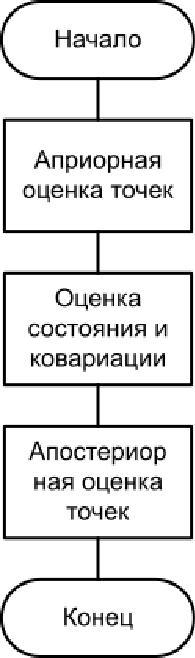
\includegraphics[height=10cm]{ukf_predict}}
\caption{Алгоритм шага предсказания UKF}
\label{fig:ukf_predict}
\end{figure}

На этапе предсказания UKF генерирует набор сигма-точек на основе текущей оценки состояния и ковариации, 
пропускает их через модель системы для прогнозирования следующего состояния и ковариации.
На этапе обновления, при поступлении измерений, сигма-точки пропускаются через модель измерений, после чего вычисляются среднее измерение, 
ковариация и коэффициент усиления Калмана, используемые для корректировки состояния и ковариации с учётом новых данных.
Этот подход позволяет UKF эффективно обрабатывать нелинейности и обеспечивать точную оценку состояния.

\FloatBarrier
\begin{figure}[H]
\centering
	\fbox{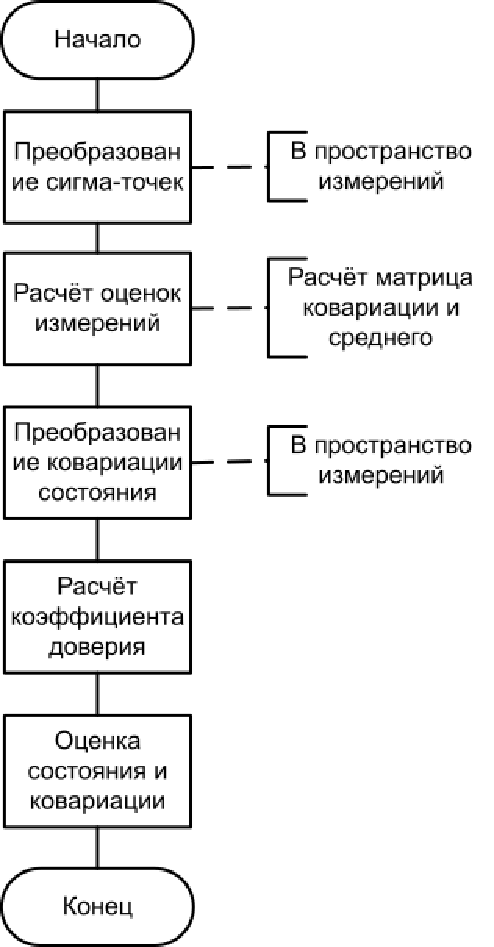
\includegraphics[height=12cm]{ukf_update}}
\caption{Алгоритм шага обновления UKF}
\label{fig:ukf_update}
\end{figure}

\subsubsection{События обновления состояния}

Данные от датчиков формируют события изменения состояния. 
Все события изменяют состояние системы в соответствии с алгоритмом обработки событий (см. рисунок \ref{fig:handle_kf_event})

\FloatBarrier
\begin{figure}[H]
\centering
	\fbox{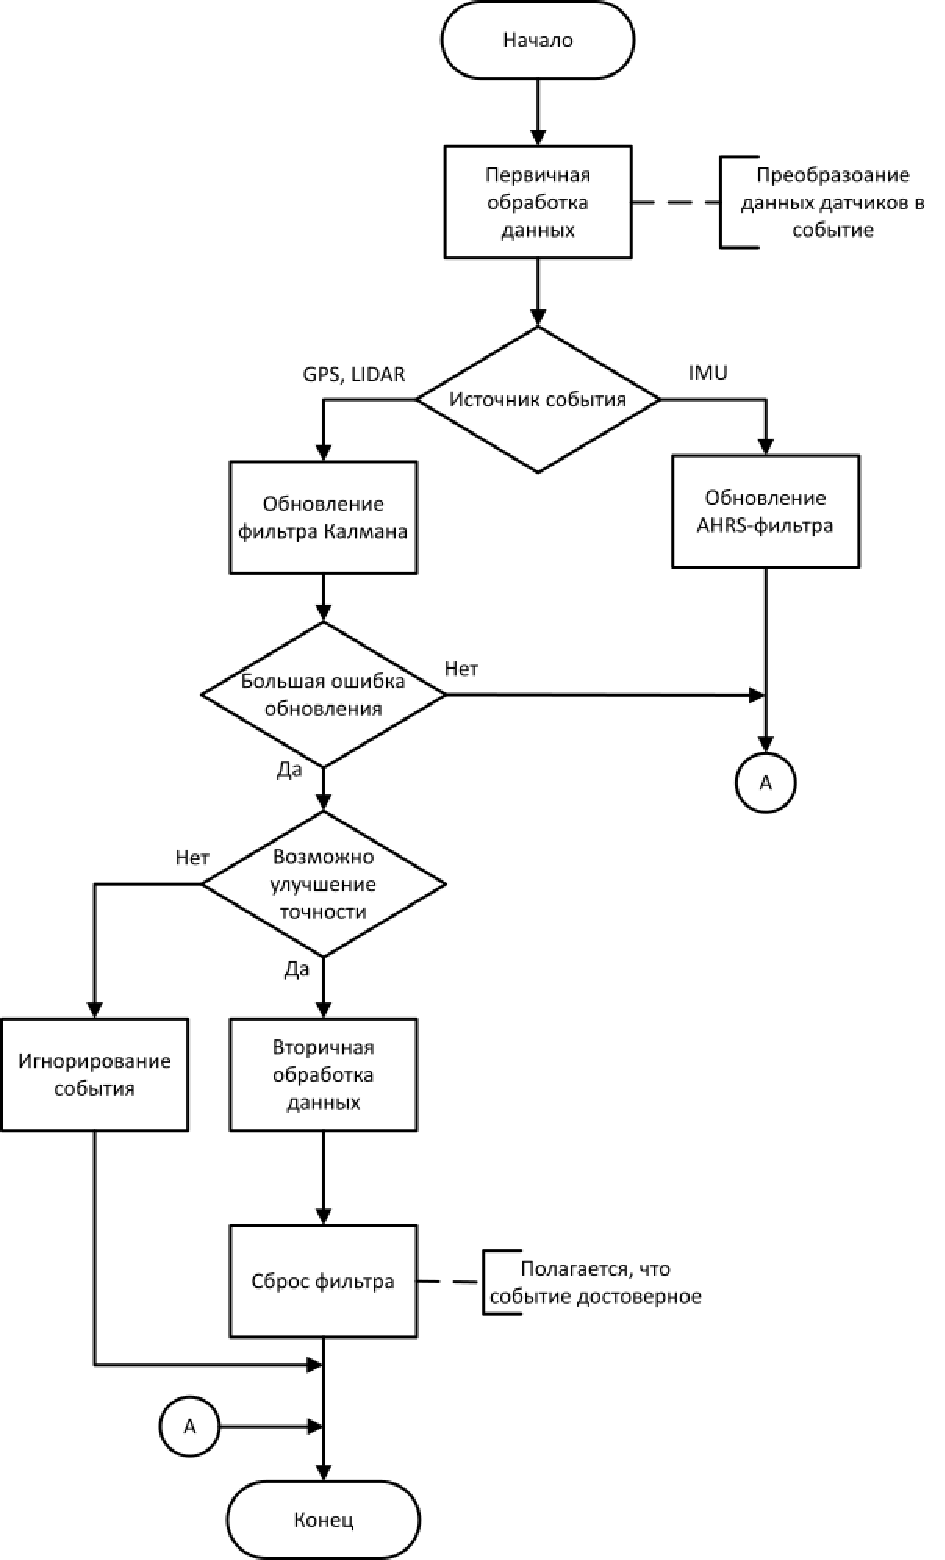
\includegraphics[height=12cm]{handle_event}}
\caption{Алгоритм обработки событий}
\label{fig:handle_kf_event}
\end{figure}


Обновление состояния в UKF выполняется только по позиционным событиям, 
которые происходят относительно редко, но обладают высокой точностью.
Позиционными событими являются содержат оценку координат робот в системе координат локальной карты робота ($x, y$) и
необязательную оценку ориентации робота в пространстве ($\theta$).
К таким событиям относятся результаты обработки данных от GPS и LIDAR.

Для обработки данных IMU используется фильтр Маджвика (см. подраздел \href{sec:ahrs}). Было принято решение использовать
отдельный фильтр для обработки данных IMU, а не обновлять вектор системы ${X}$,
по следующим причинам:
\begin{itemize}
	\item данные IMU измеряют только ориентацию, потому фильтр не сможет произвести коррекцию
	      всего вектора состояния во времени;
        \item данные от IMU приходят с гораздо большей частотой (1000 Hz), чем данные от LIDAR (10 Hz) или GPS (5 Hz).
\end{itemize}

Оценка ориентации с помощью фильтра Маджвика используется 
в процессе обработки данных LIDAR или GPS для формирования позиционных событий.

Таким образом, использованием фильтра Маджвика обеспечивает надежную и частую оценку ориентации, в то время как UKF использует редкие, но точные позиционные данные для коррекции полного вектора состояния.
Это повышает общую точность и устойчивость системы в условиях сложной динамики и возможных выбросов в измерениях.

\subsection{Очереди событий и очереди состояний}
\label{subsec:queues}

Каждое состояние системы ${X}_k$ и событие ${E}_k$ 
закреплено к моменту времени $t_k$. Каждое новое событие 
обновляет модель системы в сооветствие с алгоритмом применения события (см. рисунок \ref{fig:apply_kf_event})
\FloatBarrier
\begin{figure}[H]
\centering
	\fbox{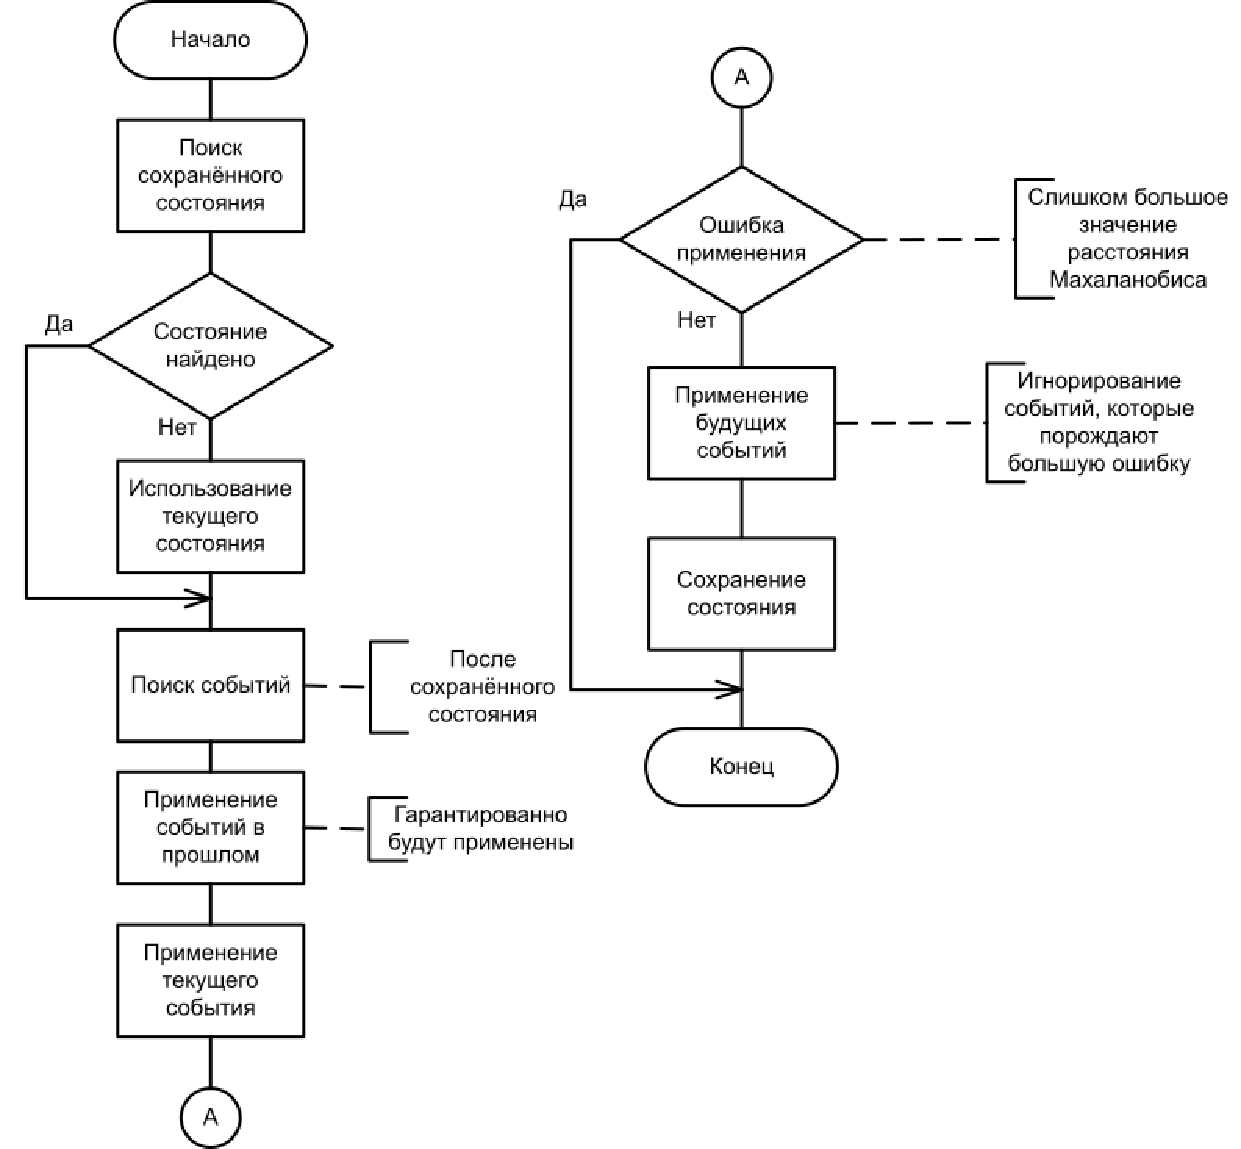
\includegraphics[height=12cm]{apply_event}}
\caption{Алгоритм применения события}
\label{fig:apply_kf_event}
\end{figure}

Для эффективной обработки данных и управления временной динамикой системы реализованы очереди состояний и событий.
Это позволяет синхронизировать данные от различных источников и корректно обновлять состояние системы в UKF.

\subsubsection{Очередь состояний}
\label{subsec:state_queue}

Очередь состояний представляет собой упорядоченный набор векторов состояния системы.
Основные характеристики очереди состояний:
\begin{itemize}
    \item каждое состояние в очереди соответствует определённому моменту времени, что позволяет отслеживать эволюцию системы и выполнять ретроспективные корректировки при получении новых данных;
    \item временные метки состояний используются для сопоставления с событиями, обеспечивая согласованность между предсказаниями и измерениями;
    \item при поступлении новых данных очередь состояний обновляется, добавляя новое состояние.
\end{itemize}

\subsubsection{Очередь событий}
\label{subsec:event_queue}

Очередь событий содержит результаты обработки данных от датчиков. Каждое из событие связано с моментом времени $t$.
События представляют собой позиционные данные, которые используются для коррекции состояния в UKF.
Основные характеристики очереди событий:
\begin{itemize}
    \item каждое событие имеет метку времени для определения положения относительно текущего момента времени;
    \item относительно события с временем $t_{\text{current}}$ события разделяются на события прошлого и события будущего;
    \item события прошлого используются для ретроспективной коррекции состояний, если данные поступили с задержкой или требуется уточнение предыдущих оценок;
    \item события будущего хранятся в очереди для обработки по мере продвижения текущего времени системы. Это позволяет системе быть готовой к асинхронным данных.
    \item очередь событий поддерживает асинхронное поступление данных от датчиков с разной частотой. 
\end{itemize}

\subsection{Планирование движения}


\subsubsection{Локальный планировщик}

В качестве локального планировщика используется DWA.
Целевая функция:
\begin{equation}
	G(v, \omega) = \sum_{i=1}^k w_i \cdot g_{i, \text{norm}}(v, \omega),
\end{equation}
где $g_{i,\text{norm}}(v, \omega)$ -- значение $i$-й подцелевой функции,
$w_i$ -- весовой коэффициент,
настраиваемый для задания приоритетов, а $k$ -- количество метрик.

Для обеспечения сравнимости метрик,
имеющих разные единицы измерения и диапазоны,
значения подцелевых функций $g_i(v, \omega)$ нормализуются по всем возможным парам скоростей 
в динамическом окне $V_d$.
Нормализованное значение вычисляется как:
\begin{equation}
	g_{i, \text{norm}}(v, \omega) = \frac{g_i(v, \omega) - \min_{(v', \omega') \in V_d} g_i(v', \omega')}{\max_{(v', \omega') \in V_d} g_i(v', \omega') - \min_{(v', \omega') \in V_d} g_i(v', \omega')},
\end{equation}
где $\min_{(v', \omega') \in V_d} g_i(v', \omega')$ и $\max_{(v', \omega') \in V_d} g_i(v', \omega')$ --
минимальное и максимальное значения $i$-й подцелевой функции среди всех пар $(v', \omega')$ в $V_d$.

Нормализация приводит значения к диапазону $[0, 1]$, что позволяет весам $w_i$ эффективно управлять
приоритетами метрик и обеспечивает сбалансированную оценку траекторий.

Для каждой пары скоростей предлагается построение уникальной траектории.
Оценка происходит не столько по значениями скорости, сколько по траекториям, которые скорости генерируют.
В качестве метрик предлагается использовать:
\begin{enumerate}
    \item Метрика близости к цели. Чем ближе конечная точка траектория к цели, 
	    тем траектория приоритетнее.
    \item Метрика близости к глобальной траектории. Чем ближе форма траектории к прямолинейной форме траектории,
	    тем траектория приоритетнее.  
    \item Метрика избегания препятствий. Приоритет отдаётся тем траектории, 
	    которые проходят дальше от препятствий.
    \item Метрика колебательных движений. Предотвращает резкие (осциллирующие) изменения скоростей 
	    для обеспечения плавности и зацикливания.
    \item Выравнивание по целевой ориентации. 
	    Минимизирует отклонение ориентации робота от желаемого угла в целевой точке.
    \item Метрика коллизий. Отклоняет все траектории, 
	    в которых обнаружены столкновения с объектами препятствий.
\end{enumerate}

% \subsubsection{Применение}

% \subsubsection{Глобальный планировщик}

\subsection{Взаимодействие с периферией}


В процессе разработки программного обеспечения для автономной навигации
мобильных платформ одной из ключевых задач стало обеспечение гибкого и надёжного
взаимодействия с периферийными устройствами, такими как датчики, камеры и
лидары. После анализа различных подходов было принято решение реализовать это
взаимодействие с использованием стека протоколов TCP/IP. Такой выбор обусловлен
универсальностью и стандартизацией данного протокола, который широко применяется
в сетевых технологиях и позволяет организовать стабильное соединение между
компонентами системы. Это решение обеспечивает возможность передачи данных в
реальном времени, что критически важно для задач управления и обработки
информации в динамичной среде.

Использование TCP/IP стека предоставляет значительное преимущество в виде
модульности и расширяемости системы. Благодаря этому подходу стало возможным
подключение различных датчиков к программе непосредственно во время её работы,
без необходимости останавливать или перезапускать систему. Например, если в
процессе эксплуатации мобильной платформы потребуется добавить новый лидар или
ультразвуковой датчик, это можно сделать "на лету", что существенно повышает
адаптивность системы к изменяющимся условиям или требованиям задачи. Такая
гибкость особенно ценна в экспериментальных или полевых условиях, где заранее
предусмотреть все сценарии использования невозможно.

Реализация взаимодействия через TCP/IP также упрощает интеграцию с современными
технологиями и стандартами, используемыми в робототехнике. Например, многие
устройства уже имеют встроенную поддержку сетевых протоколов, что позволяет
избежать разработки сложных проприетарных интерфейсов для каждого типа
периферии. Кроме того, TCP/IP обеспечивает надёжную передачу данных с механизмом
проверки ошибок, что снижает риск потери критически важной информации от
датчиков. Это особенно актуально для автономных систем, где точность и
своевременность получения данных напрямую влияют на качество навигации и
принятия решений.

Наконец, выбор TCP/IP стека открывает перспективы для дальнейшего развития
проекта в сторону распределённых систем. В будущем это позволит не только
подключать датчики локально, но и организовывать взаимодействие между
несколькими мобильными платформами или центральным сервером через сеть. Такой
подход может быть полезен, например, для координации группы роботов или передачи
данных в облако для анализа. Таким образом, использование TCP/IP не только
решает текущие задачи взаимодействия с периферией, но и закладывает фундамент
для масштабирования системы, делая её более универсальной и готовой к новым
вызовам в области автономной навигации.

\subsection{Язык программирования}
Robot Operating System (ROS) представляет собой широко используемую программную
платформу для разработки робототехнических систем, и одной из её ключевых
особенностей является то, что она написана на языке программирования C++. Этот
выбор не случаен: C++ считается стандартом индустрии благодаря своей высокой
производительности, гибкости и возможности работы на низком уровне с аппаратным
обеспечением. В контексте робототехники, где требуется быстрая обработка данных
с датчиков и управление механизмами в реальном времени, такие качества C++
становятся незаменимыми. Использование C++ в ROS позволяет разработчикам
создавать эффективные и масштабируемые решения для сложных задач, таких как
автономная навигация, обработка сигналов или взаимодействие с физическими
устройствами. Этот язык обеспечивает тонкий контроль над ресурсами системы, что
особенно важно для мобильных платформ с ограниченными вычислительными
мощностями. Кроме того, C++ обладает богатым набором библиотек и инструментов,
которые упрощают интеграцию ROS с другими технологиями, укрепляя его как
стандарта в индустрии робототехники.

Несмотря на все преимущества C++ как стандарта индустрии и основы для ROS, в
последние годы всё большее внимание в разработке программного обеспечения,
включая робототехнику, привлекает язык программирования Rust. В контексте ROS
уже появляются инициативы по интеграции Rust, что может дополнить или даже со
временем частично заменить C++, предлагая разработчикам более надёжный и удобный
инструмент для создания автономных систем, сохраняя при этом совместимость с
существующей экосистемой ROS.

Одним из ключевых преимуществ Rust является его способность обеспечивать
безопасность многозадачности. В отличие от C++, который требует дополнительных
усилий для безопасного выполнения параллельных операций, Rust изначально
предусматривает механизмы предотвращения гонок данных, что делает код более
надежным. Это особенно важно для системы навигации, где необходимо параллельно
обрабатывать данные с различных сенсоров и вычислять управляющие команды без
риска возникновения ошибок синхронизации.

Rust также предоставляет встроенные инструменты для работы с асинхронным
программированием, что позволяет эффективно организовать обработку данных в
реальном времени. Асинхронные операции позволяют системе собирать данные с
сенсоров, планировать маршрут и управлять моторами без блокировки основного
потока выполнения, что способствует повышению производительности и снижению
задержек.

Программная экосистема Rust активно развивается, и существует множество
библиотек, которые могут быть использованы для решения задач, связанных с
обработкой сенсорных данных, математическими расчетами и оптимизацией маршрутов.
Это позволяет разработчикам легко интегрировать необходимые инструменты и
сокращать время на разработку и тестирование системы. Также, благодаря хорошей
поддержке со стороны сообщества, Rust предоставляет разработчикам множество
ресурсов для быстрого решения возникающих вопросов.

Ключевым преимуществом Rust является его кроссплатформенность. Код, написанный
на этом языке, может быть скомпилирован для различных платформ, что делает Rust
отличным выбором для мобильных роботов, которые могут работать на разных типах
оборудования. Это позволяет без значительных усилий адаптировать систему под
разные архитектуры и аппаратные платформы.

Будущие улучшения системы могут включать в себя добавление новых сенсоров,
улучшение алгоритмов SLAM и маршрутизации, а также интеграцию с внешними
системами, такими как онлайн-карты или системы для прогнозирования дорожной
ситуации. Rust, благодаря своей гибкости и безопасному управлению памятью,
идеально подходит для такой работы, обеспечивая долгосрочную устойчивость и
развитие проекта.

Таким образом, проектирование программного обеспечения для системы мобильной
навигации с использованием сенсоров и алгоритмов SLAM требует тщательной
проработки архитектуры, выбора эффективных технологий и инструментов. Язык Rust
является отличным выбором для разработки таких систем, благодаря своим
преимуществам в безопасности, производительности и поддержке многозадачности,
что делает его идеальным для создания высоконадежных и высокопроизводительных
приложений для робототехники.

Robot Operating System (ROS) представляет собой широко используемую программную
платформу для разработки робототехнических систем, и одной из её ключевых
особенностей является то, что она написана на языке программирования C++. Этот
выбор не случаен: C++ считается стандартом индустрии благодаря своей высокой
производительности, гибкости и возможности работы на низком уровне с аппаратным
обеспечением. В контексте робототехники, где требуется быстрая обработка данных
с датчиков и управление механизмами в реальном времени, такие качества C++
становятся незаменимыми. Использование C++ в ROS позволяет разработчикам
создавать эффективные и масштабируемые решения для сложных задач, таких как
автономная навигация, обработка сигналов или взаимодействие с физическими
устройствами. Этот язык обеспечивает тонкий контроль над ресурсами системы, что
особенно важно для мобильных платформ с ограниченными вычислительными
мощностями. Кроме того, C++ обладает богатым набором библиотек и инструментов,
которые упрощают интеграцию ROS с другими технологиями, укрепляя его как
стандарта в индустрии робототехники.

Несмотря на все преимущества C++ как стандарта индустрии и основы для ROS, в
последние годы всё большее внимание в разработке программного обеспечения,
включая робототехнику, привлекает язык программирования Rust. В контексте ROS
уже появляются инициативы по интеграции Rust, что может дополнить или даже со
временем частично заменить C++, предлагая разработчикам более надёжный и удобный
инструмент для создания автономных систем, сохраняя при этом совместимость с
существующей экосистемой ROS.

Одним из ключевых преимуществ Rust является его способность обеспечивать
безопасность многозадачности. В отличие от C++, который требует дополнительных
усилий для безопасного выполнения параллельных операций, Rust изначально
предусматривает механизмы предотвращения гонок данных, что делает код более
надежным. Это особенно важно для системы навигации, где необходимо параллельно
обрабатывать данные с различных сенсоров и вычислять управляющие команды без
риска возникновения ошибок синхронизации.

Rust также предоставляет встроенные инструменты для работы с асинхронным
программированием, что позволяет эффективно организовать обработку данных в
реальном времени. Асинхронные операции позволяют системе собирать данные с
сенсоров, планировать маршрут и управлять моторами без блокировки основного
потока выполнения, что способствует повышению производительности и снижению
задержек.

Программная экосистема Rust активно развивается, и существует множество
библиотек, которые могут быть использованы для решения задач, связанных с
обработкой сенсорных данных, математическими расчетами и оптимизацией маршрутов.
Это позволяет разработчикам легко интегрировать необходимые инструменты и
сокращать время на разработку и тестирование системы. Также, благодаря хорошей
поддержке со стороны сообщества, Rust предоставляет разработчикам множество
ресурсов для быстрого решения возникающих вопросов.

Ключевым преимуществом Rust является его кроссплатформенность. Код, написанный
на этом языке, может быть скомпилирован для различных платформ, что делает Rust
отличным выбором для мобильных роботов, которые могут работать на разных типах
оборудования. Это позволяет без значительных усилий адаптировать систему под
разные архитектуры и аппаратные платформы.

Будущие улучшения системы могут включать в себя добавление новых сенсоров,
улучшение алгоритмов SLAM и маршрутизации, а также интеграцию с внешними
системами, такими как онлайн-карты или системы для прогнозирования дорожной
ситуации. Rust, благодаря своей гибкости и безопасному управлению памятью,
идеально подходит для такой работы, обеспечивая долгосрочную устойчивость и
развитие проекта.

Таким образом, проектирование программного обеспечения для системы мобильной
навигации с использованием сенсоров и алгоритмов SLAM требует тщательной
проработки архитектуры, выбора эффективных технологий и инструментов. Язык Rust
является отличным выбором для разработки таких систем, благодаря своим
преимуществам в безопасности, производительности и поддержке многозадачности,
что делает его идеальным для создания высоконадежных и высокопроизводительных
приложений для робототехники.
